\documentclass[ a4paper, 12pt]{report}
%
\usepackage[text={16cm,24cm},centering]{geometry} % geometrija stranice
\usepackage[utf8]{inputenc}
\usepackage[croatian]{babel}
\usepackage{amssymb ,amsmath, amsthm}
\usepackage{graphicx} % paket za umetanje slika
%\usepackage{psfrag} % paket za pisanje po slikama
\usepackage{ccaption} % paket za kontroliranje "caption"-a za table, figure, ...
%
\newtheorem{defn}{Definicija}[section]
\newtheorem{tm}{Teorem}[section]
\newtheorem{prop}{Propozicija}[section]
\newtheorem{lm}{Lema}[section]
\newtheorem{cor}{Korolar}[tm]
%
\renewcommand{\thechapter}{\Roman{chapter}}
\renewcommand{\thesection}{\arabic{section}}
\renewcommand{\theequation}{\arabic{section}.\arabic{equation}}
\renewcommand{\thefigure}{\arabic{section}.\arabic{figure}}
%  za detaljnije informacije o numeriranju
%  mozete pogledati npr.
%  http://www.iam.ubc.ca/~newbury/tex/numbering.html
%
\flushbottom
\addtolength{\voffset}{-0.5cm}
%\renewcommand{\baselinestretch}{2}
%  odkomentirajte ako zelite dvostruki prored
%
\captiondelim{}
%  ako necete imati, kod slika ili tablica, captione
%  npr: samo "Slika 1" a ne "Slika 1: Nesto"
%  inace zakomentirajte
%
\newcommand{\bi}[1]{\textbf{\em{#1}}}
% naredba "\bi{nesto}" tekst nesto stavlja u bold i italic
%
\newcounter{Section}
\setcounter{Section}{0}
%
\newcommand{\Section}[1]{ \section{#1}
  \setcounter{figure}{0} \setcounter{equation}{0}
  \addtocounter{Section}{1} }
% Napomena: section zapocinjite s \Section{...} a ne \section{...}
%
\newcommand{\Chapter}[1]{ \chapter{#1}
  \setcounter{section}{\value{Section}} }
% Napomena: chapter zapocinjite s \Chapter{...} a ne \chapter{...}
%
%\includeonly{}
%  odkomentirajte ako zelite da se kompajlira samo Sazetak + Poglavlja
%  u \includeonly{} mozete dodati sve sto se includa u ovoj datoteci
%
%%%%%%%%%%%%%%%%%%%%%%%%%%%%%%%%%%%%%%%
% Informacije potrebne za naslovnicu.
% Mogu se koristiti i izvan naslovnice.
%
\newcommand{\Fakultet}{
  Sveu\v{c}ili\v{s}te u Zagrebu \\[5mm]
  PMF - Matemati\v{c}ki odjel
}
\newcommand{\ImePrezimeAutora}{Ime i Prezime}
\newcommand{\NaslovRada}{Naslov rada}
\newcommand{\ImePrezimeMentora}{prof. dr. sc. Ime i Prezime}
\newcommand{\MjestoDatum}{Zagreb, mjesec godina}
%
%%%%%%%%%%%%%%%%%%%%%%%%%%%%%%%%%%%%%%%%%%%%%%%%%%%%%%%%%%%%%%%%%%%%%%%%%%%%%%%%
%%%%%%%%%%%%%%%%%%%%%%%%%%%%%%%%%%%%%%%%%%%%%%%%%%%%%%%%%%%%%%%%%%%%%%%%%%%%%%%%
% Pocetak dokumenta
%
\begin{document}
%
%%%%%%%%%%%%%%%%%%%%%%%%%%%%%%%%%%%%
% Naslovnica diplomskog rada
%%%%%%%%%%%%%%%%%%%%%%%%%%%%%%%%%%%%
%
\thispagestyle{empty}
%
\begin{center}
  \Large{
    \Fakultet
  }
\end{center}
\vskip 150pt
\begin{center}
  \LARGE{
    \lineskip .75em
    \begin{tabular}[t]{c}
      \ImePrezimeAutora
    \end{tabular}
    \par
  }
  \vskip 3em
  \huge{
    \NaslovRada
    \par
  }
  \vskip 3em
  \Large{
    Diplomski rad
  }
\end{center}
\par
%
\vskip 125pt
\vfill
%
\begin{center}
  \large{
    \MjestoDatum
    \par
  }
\end{center}
%
\newpage
%
\thispagestyle{empty}
%
\begin{center}
  \Large{
    \Fakultet
  }
\end{center}
\vskip 150pt
\begin{center}
  \LARGE{
    \lineskip .75em
    \begin{tabular}[t]{c}
      \ImePrezimeAutora
    \end{tabular}
    \par
  }
  \vskip 3em
  \huge{
    \NaslovRada
    \par
  }
  \vskip 3em
  \Large{
    Diplomski rad
  }
\end{center}
\par
%
\vskip 125pt
\mbox{} \hfill
%
\begin{minipage}{8cm}
  \Large{
    Voditelj rada:\\
    \hspace*{10pt}
    \ImePrezimeMentora
  }
\end{minipage}
%
\vfill
%
\begin{center}
  \large{
    \MjestoDatum
    \par
  }
\end{center}
%

%%%%%%%%%%%%%%%%%%%%%%%%%%%%%%%%%%%%%%%%%%
% Povjerenstvo i ocjene, sluzbeni oblik
%%%%%%%%%%%%%%%%%%%%%%%%%%%%%%%%%%%%%%%%%%
%
\thispagestyle{empty}
%
Ovaj diplomski rad obranjen je dana
\begin{tabular}{p{5.0 cm}}
\\
\hline
\end{tabular}
pred nastavni\v{c}kim povjerenstvom
u sastavu:
%
\vskip 30pt
\begin{enumerate}
\item{
\begin{tabular}{p{7.0 cm}}

\\
\hline
\end{tabular}
, predsjednik
}
\vskip 20pt
\item{
\begin{tabular}{p{7.0 cm}}
\\
\hline
\end{tabular}
, \v{c}lan
}
\vskip 20pt
\item{
\begin{tabular}{p{7.0 cm}}
\\
\hline
\end{tabular}
, \v{c}lan
}
\end{enumerate}
\vskip 25pt
%
Povjerenstvo je rad ocijenilo ocjenom
\begin{tabular}{p{5.0 cm}}
\\
\hline
\end{tabular}.
\vskip 25pt
%
Potpisi \v{c}lanova povjerenstva:
\vskip 30pt
%
\begin{enumerate}
\item{
\begin{tabular}{p{7.0 cm}}
\\
\hline
\end{tabular}
} %\item
\vskip 30pt
\item{
\begin{tabular}{p{7.0 cm}}
\\
\hline
\end{tabular}
} %\item
\vskip 30pt
\item{
\begin{tabular}{p{7.0 cm}}
\\
\hline
\end{tabular}
} %\item
\end{enumerate}


%
%%%%%%%%%%%%%%%%%%%%%%%%%%%%%%%%%%%%%%%%%%%%%
% Sadrzaj
%
\newpage
\pagenumbering{roman} \setcounter{page}{1}
\tableofcontents
%
%%%%%%%%%%%%%%%%%%%%%%%%%%%%%%%%%%%%%%%%%%%%%
%%%%%%%%%%%%%%%%%%%%%%%%%%%%%%%%%%%%%%%%%%%%%
%
%%%%%%%%%%%%%%%%%
% Uvod
%%%%%%%%%%%%%%%%%
%
\chapter*{Uvod}
\addcontentsline{toc}{chapter}{Uvod}
%
%%%%%%%%%%%%%%%%%%%%%%%%%%%%%%%%%%%%%%%%%%%
% Ovdje napisite uvod

\v{C}esto nas zanima konvergira li 
neki niz slu\v{c}ajnih varijabli po distribuciji te,
ukoliko konvergira, prema kojoj distribuciji.
Osim teorijskih vrijednosti ovakvi su rezultati
zna\v{c}ajni i u prakti\v{c}noj primjeni.
U ovom \'{c}emo radu pokazati da su Wilcoxonove
statistike sume rangova (eng. \textit{Wilcoxon rank-sum
statistic}) i rangova s predznacima (eng.
\textit{Wilcoxon signed-rank statistic})
asimptotski normalne (te\v{z}e po distribuciji
prema normalnoj razdiobi) uz odre\dj{}ene uvjete.


%
\pagenumbering{arabic} \setcounter{page}{1}
%
%%%%%%%%%%%%%%%%%%%%%%%%%%%%%%%%%%%%%%%%%%%%%
% Ovdje napisite naziv prvog poglavlja
\Chapter{Naziv prvog poglavlja}
%%%%%%%%%%%%%%%%%%%%%%%%%%%%%%%%%%%%%%%%%%%%%
%
%%%%%%%%%%%%%%%%%%%%%%%%%%%%%%%%%%%%%%%%%%%
% Ovdje napisite naziv prvog Sectiona
\Section{Prvi naslov} \label{Sec:1}
%
% Ispod napisite tekst Sectiona

% Na primjer
Za bilo koji homogeni polinom $F(x,y,z)$ neka je $f(x,y)=F(x,y,1)$. Tada iz
jednad\v{z}be 1.5 dobivamo
$$f(x,y)=\sum e_{ij} x^i y^j \mathrm{.}$$
To\v{c}ka euklidske ravnine $(x,y)$ le\v{z}i na grafu od $f(x,y)=0$ ako i samo ako odgovaraju\'{c}a
to\v{c}ka projektivne ravnine $(x,y,1)$ le\v{z}i na grafu od $F(x,y,z)=0$. Dakle, krivulje
$f=0$ i $F=0$ sadr\v{z}e iste to\v{c}ke euklidske ravnine pa $f$ zovemo \bi{restrikcijom}
krivulje $F$.

%%%%%%%%%%%%%%%%%%%%%%%%%%%%%%%%%%%%%%%%%%%
% Ovdje napisite naziv drugog Sectiona
\Section{Drugi naslov} \label{Sec:2}
%
% Ispod napisite tekst Sectiona

% Na primjer
\begin{equation}
F(x,y,1)=f(x,y) \mathrm{.}
\end{equation}
Sada je o\v{c}ito da $F=0$ i $f=0$ sadr\v{z}e iste to\v{c}ke euklidske ravnine. Krivulju $F=0$
zovemo \bi{pro\v{s}irenje} krivulje $f$ u projektivnu ravninu ili jednostavnije pro\v{s}irenje
od $f$.

Broj presjeka izme\dj{}u dvije krivulje u ishodi\v{s}tu ne bi
se trebao promijeniti ako krivulju restriktiramo iz projektivne ravnine u
euklidsku ravninu i zamjenimo homogene koordinate sa uobi\v{c}ajnim $(x,y)$ koordinatama.


%
%
%%%%%%%%%%%%%%%%%%%%%%%%%%%%%%%%%%%%%%%%%%%%%
% Ovdje napisite naziv drugog poglavlja
\Chapter{Naziv drugog poglavlja}
%%%%%%%%%%%%%%%%%%%%%%%%%%%%%%%%%%%%%%%%%%%%%
%
%%%%%%%%%%%%%%%%%%%%%%%%%%%%%%%%%%%%%%%%%%%
% Ovdje napisite naziv treceg Sectiona
\Section{Tre\'{c}i naslov} \label{Sec:3}
%
% Ispod napisite tekst Sectiona

% Na primjer
\begin{tm}[Pappusov teorem \cite{PJRyan+EaNEG}]
Neka su e i f dva pravca koji le\v{z}e u projektivnoj ravnini. Neka su A, B i C to\v{c}ke koje le\v{z}e
na pravcu $e$, razli\v{c}ite od to\v{c}ke $e \cap f$ i neka su $A'$, $B'$ i $C'$ tri to\v{c}ke pravca $f$
razli\v{c}ite od to\v{c}ke $e \cap f$. Tada su to\v{c}ke $Q=AB' \cap A'B$, $R=BC' \cap B'C$ i
$S=CA' \cap C'A$ kolinearne.
\end{tm}
%
\begin{figure}[!ht]
\begin{center}
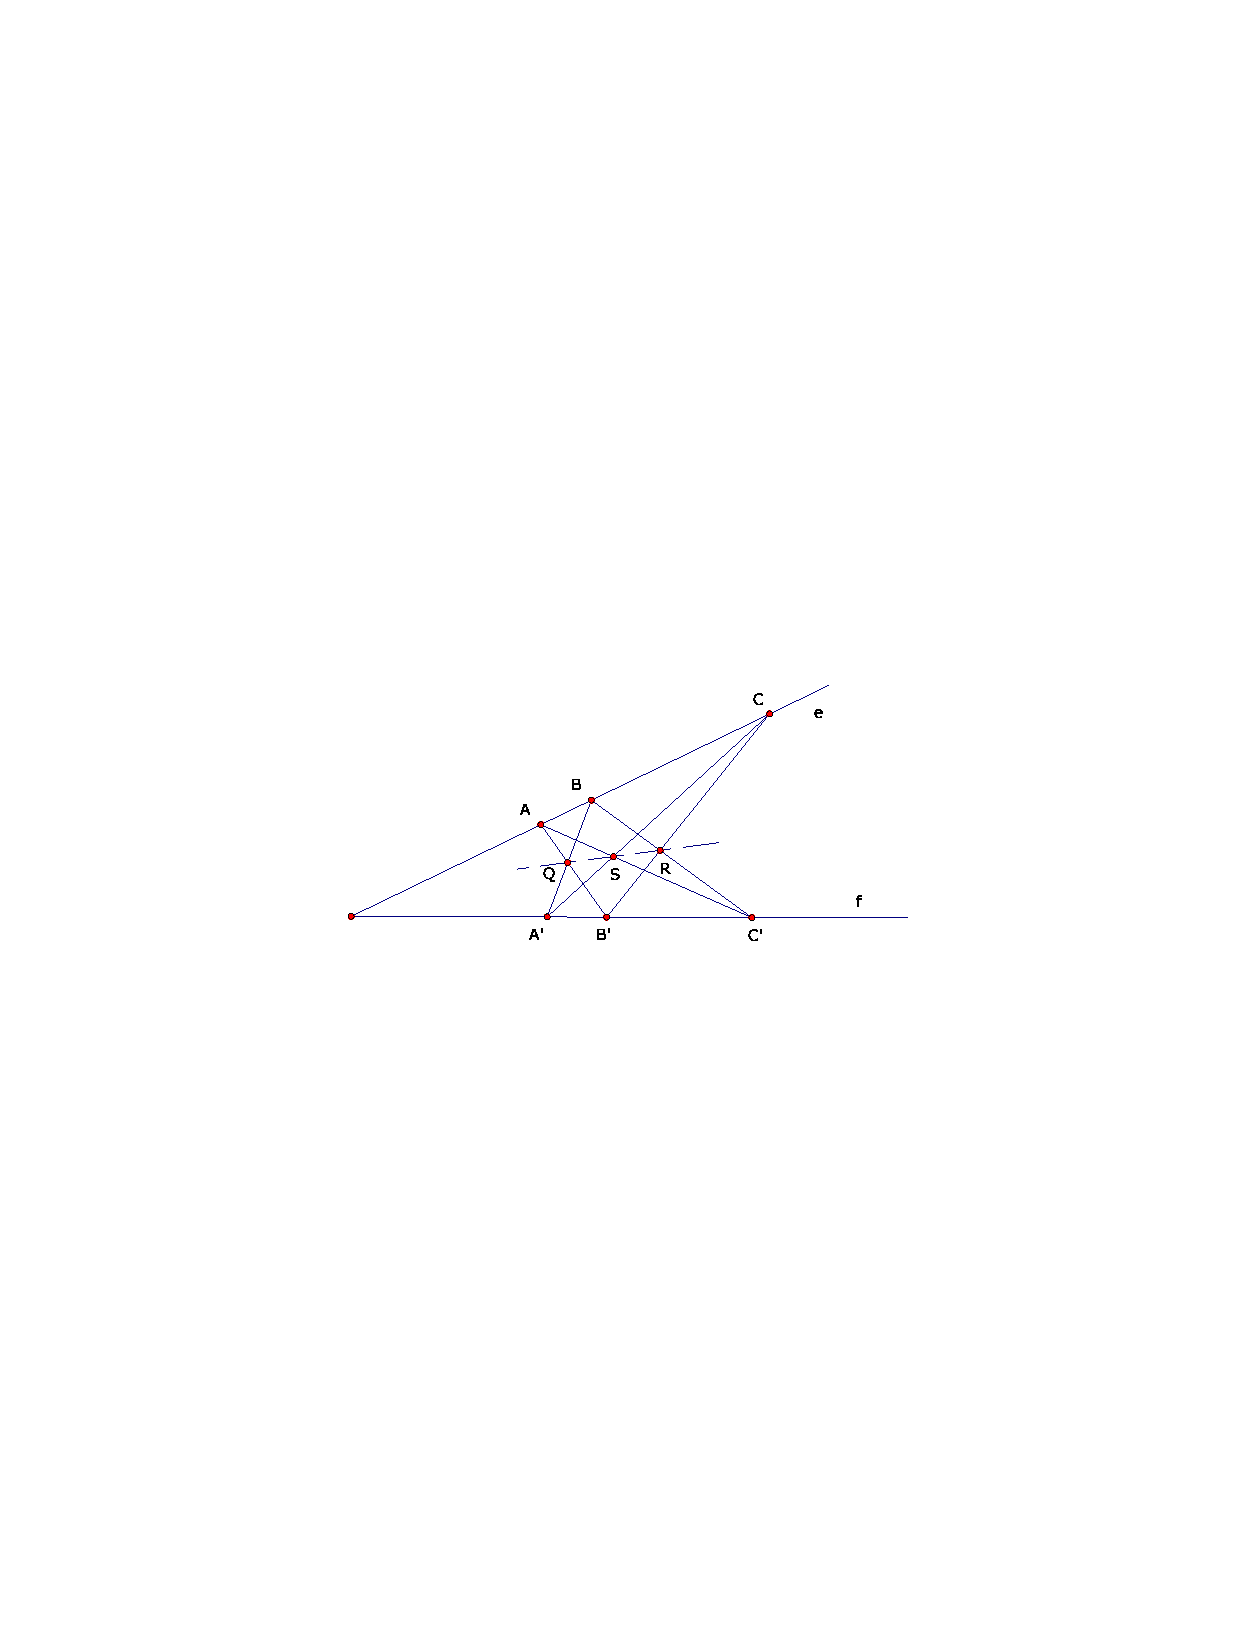
\includegraphics[clip, viewport=150 320 440 460]{slike/slika_3-1.eps}
\caption{}
\label{fig:3.1}
\end{center}
\end{figure}


%
%%%%%%%%%%%%%%%%%%%%%%%%%%%%%%%%%%%%%%%%%%%%%
%%%%%%%%%%%%%%%%%%%%%%%%%%%%%%%%%%%%%%%%%%%%%
%
%%%%%%%%%%%%%%%%%
% Zakljucak
%%%%%%%%%%%%%%%%%
%
\chapter*{Zaklju\v{c}ak}
\addcontentsline{toc}{chapter}{Zaklju\v{c}ak}
%
%%%%%%%%%%%%%%%%%%%%%%%%%%%%%%%%%%%%%%%%%%%
% Ovdje napisite zakljucak

Lagani zaklju\v{c}ak ...

%%%%%%%%%%%%%%%%%%%%%%%%%%%%%%%%%%%%%%
% Osnovni parametri za bibliografiju
%
\nocite{*}
\bibliography{bibliografija/diplomski_bibliografija}
\bibliographystyle{plain}

%
\end{document}

